\documentclass{beamer}
\usepackage{enumitem}
\usepackage{tikz}
\usetikzlibrary{circuits.logic.US,calc}
\usetheme{Boadilla}


\title{My Presentation For Assignmnet 11}
\subtitle{Assignmnet}
\author{ABHYUDAY CHOUMAL}
\institute{IIIT RAICHUR}
\date{\today}
\begin{document}
 <presentation>
 
 \titlepage start:


 
 \section{Section 1}
\subsection{sub a}

\begin{frame}
\frametitle{PROBLEM STATMENT :}
(Q.1)  
      A bulb in a stair case has two switches, one switch being at the ground floor and the other one at the first floor.The bulb can be turned ON and also can be turned OFF by any one of the switches irrespective of the state of the other switch the logic in switching of the bulb resembles.

\begin{enumerate}[label=(\Alph*)]
\item an AND gate
\item an OR gate
\item an XOR gate
\item an NAND gate
\end{enumerate}


\end{frame}
 
 \begin{frame}
\frametitle{ANSWER:-}
 \framesubtitle{ANSWER BY OPTION }
		the answer to the given question is (c)= XOR GATE
 
 \end{frame}
 
  \begin{frame}
\frametitle{XOR GATE FOR PROBLEM SOLVING :}
 
  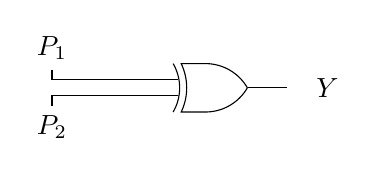
\begin{tikzpicture}[circuit logic US]
\draw (0,0) node[xor gate](XOR1){}
  
  (XOR1.input 1) -- ++(-.5,0)
 
  (XOR1.input 2) -- ++(-.5,0)
  
  (XOR1.output) -- ++(.5,0);

\node (x1) at (-2,0.5) {$P_1$};
\node (x2) at (-2,-0.5) {$P_2$};
\node (x3) at (1.5,0) {$Y$};


\draw (x1) |- (XOR1.input 1);
\draw (x2) |- (XOR1.input 2);
    
\end{tikzpicture}
	    
	    
	    FIGURE:-1 XOR GATE
 
 
 \end{frame}
 
   \begin{frame}
\frametitle{Explanation:}
  
 let the switches be P$_1$ and P$_2$\newline


\setlength{\arrayrulewidth}{1mm}
\setlength{\tabcolsep}{18pt}
\renewcommand{\arraystretch}{1.5}



\begin{tabular}{ |p{1cm}|p{1cm}|p{1cm}| }
\hline
\multicolumn{3}{|c|}{ TRUTH TABLE } \\
\hline
input($P_1$) & input($P_2$) & output(Y) \\
\hline
  0 & 0 & 0 \\
\hline
0 & 1 & 1 \\
\hline
1 & 0 & 1 \\
\hline
1 & 1 & 0  \\
\hline

\end{tabular}


\vspace{1cm}


Y = ($\overline{P_1}$)($P_2$)+($\overline{P_2}$)($P_1$) 
  
  
  
  
  \end{frame}
  
 \begin{frame}
\frametitle{Explanation:}  

From the above truth table, it can be verified that XOR logic is implemented.
So that if we  switch on at ground floor and switch off at top floor then the bulb enlighten. (vice versa is also true). Because in the XOR gate operation output comes ON when only one input is ON and other one is OFF. so we use XOR gate for this type of problem. 

  
   \end{frame}
   
   \begin{frame} 
   \frametitle{COMPLETE}
	    
	    \centering THANK YOU
	    
	   \end{frame}  
	    
\end{document}